\section{Результат работы программы}


В режиме проверки  до обучения ИНС демонстрирует абсолютную неспособность распознаванию образов (см. рис.~\ref{ris:Check}).

\begin{figure}[h]
\center{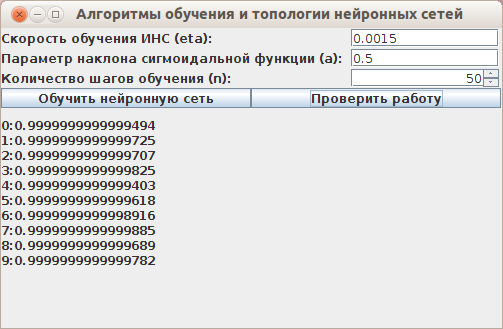
\includegraphics[width=0.75\linewidth]{check.png}}
\caption{Режим проверки до обучения.}
\label{ris:Check}
\end{figure}

Обучим нейронную сеть с различными параметрами обучения.
Проведем 50 циклов обучения сети с параметрами скорости обучения 0,0015, 0,15 и 15 (см. рис.~\ref{ris:stud_0,0015_0,5_50}, \ref{ris:stud_0,15_0,5_50} и \ref{ris:stud_15_0,5_50}).

\begin{figure}[H]
\center{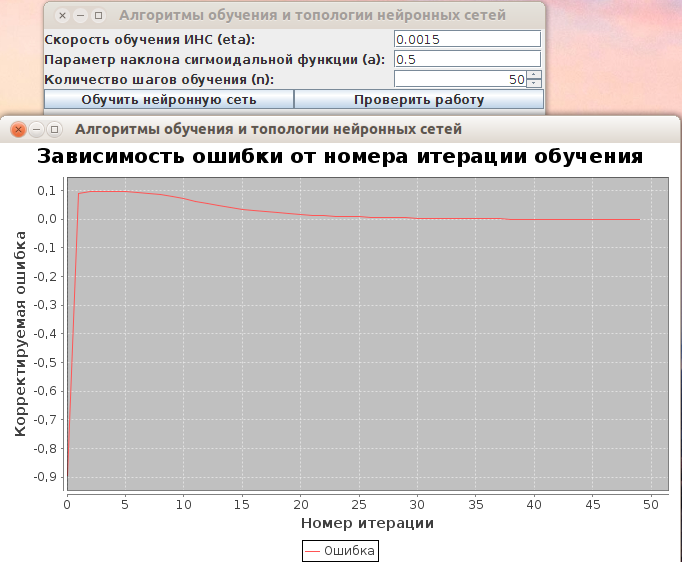
\includegraphics[width=0.75\linewidth]{stud_0,0015_0,5_50.png}}
\caption{Режим обучения. (Скорость обучения 0,0015. Параметр сигмоидальной функции 0,5. 50 циклов обучения).}
\label{ris:stud_0,0015_0,5_50}
\end{figure}

\begin{figure}[H]
\center{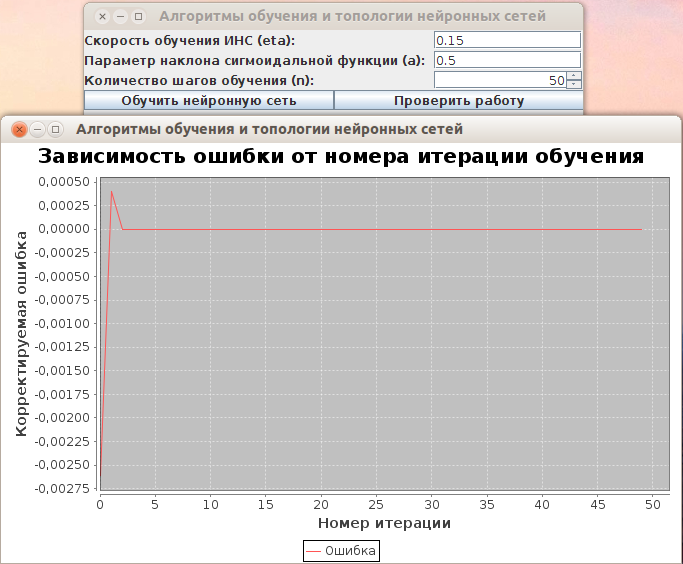
\includegraphics[width=0.75\linewidth]{stud_0,15_0,5_50.png}}
\caption{Режим обучения. (Скорость обучения 0,15. Параметр сигмоидальной функции 0,5. 50 циклов обучения).}
\label{ris:stud_0,15_0,5_50}
\end{figure}

\begin{figure}[H]
\center{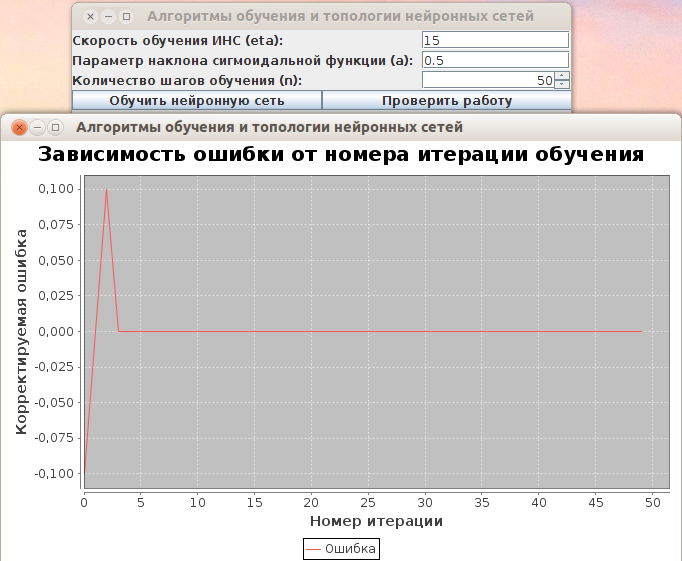
\includegraphics[width=0.75\linewidth]{stud_15_0,5_50.png}}
\caption{Режим обучения. (Скорость обучения 15. Параметр сигмоидальной функции 0,5. 50 циклов обучения).}
\label{ris:stud_15_0,5_50}
\end{figure}

Соглано полченным результатам коэффициент скорости обучения пропорционально влияет на скорость обучения. 
Однако при больших значениях возникает вероятность переобучения сети, т.е. увеличение ошибки от итерации к итерации.


Проведем 100 циклов обучения сети с параметром скорости обучения 0,0015 (см. рис.~\ref{ris:stud_0,0015_0,5_100}).

\begin{figure}[h]
\center{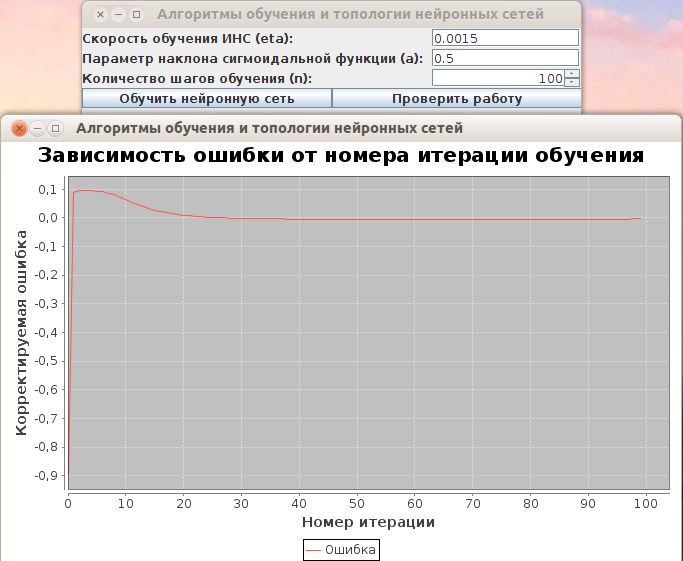
\includegraphics[width=0.75\linewidth]{stud_0,0015_0,5_100.png}}
\caption{Режим обучения. (Скорость обучения 0,0015. Параметр сигмоидальной функции 0,5. 100 циклов обучения).}
\label{ris:stud_0,0015_0,5_100}
\end{figure}

Согласно этим результатам ошибка нейронной сети уменьшается с каждой итерацией обучения.

Проведем 50 циклов обучения сети с параметром скорости обучения 0,0015 и коэффициентами наклона сигмоидальной функции 0,5 и 2,0, а затем проверим работу сети (рис.~\ref{ris:check_0,0015_0,5_50} и \ref{ris:check_0,0015_2,0_50}).

\begin{figure}[h]
\center{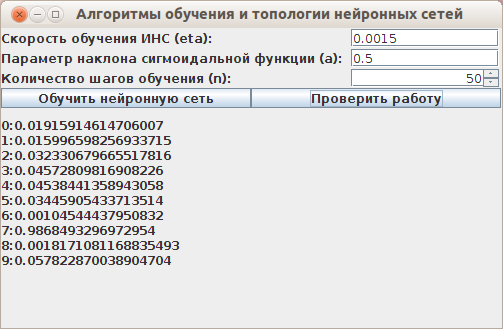
\includegraphics[width=0.75\linewidth]{check_0,0015_0,5_50.png}}
\caption{Режим проверки. (Скорость обучения 0,0015. Параметр сигмоидальной функции 0,5. 50 циклов обучения).}
\label{ris:check_0,0015_0,5_50}
\end{figure}

\begin{figure}[h]
\center{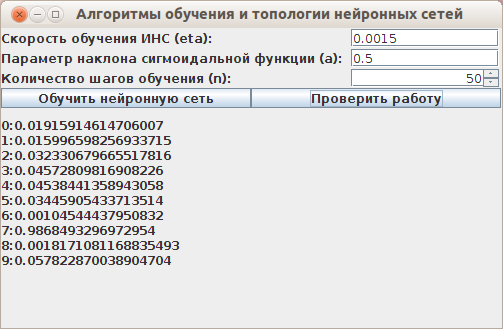
\includegraphics[width=0.75\linewidth]{check_0,0015_0,5_50.png}}
\caption{Режим проверки. (Скорость обучения 0,0015. Параметр сигмоидальной функции 2,0. 50 циклов обучения).}
\label{ris:check_0,0015_2,0_50}
\end{figure}

По результатам проверки видно, что коэффициент наклона сигмоидальной функции влияет на допустимые погрешности работы сети. Чем меньше этот коэффициент, тем сильнее сигмоидальная функция стремиться к пороговой.




